% \LaTeX-Main\
%% The LaTeX package tcolorbox - version 5.1.1 (2022/06/24)
%% tcolorbox-tutorial-poster.tex: a tutorial for poster creation with tcolorbox
%%
%% -------------------------------------------------------------------------------------------
%% Copyright (c) 2006-2022 by Prof. Dr. Dr. Thomas F. Sturm <thomas dot sturm at unibw dot de>
%% -------------------------------------------------------------------------------------------
%%
%% This work may be distributed and/or modified under the
%% conditions of the LaTeX Project Public License, either version 1.3
%% of this license or (at your option) any later version.
%% The latest version of this license is in
%%   http://www.latex-project.org/lppl.txt
%% and version 1.3 or later is part of all distributions of LaTeX
%% version 2005/12/01 or later.
%%
%% This work has the LPPL maintenance status `author-maintained'.
%%
%% This work consists of all files listed in README
%%
% arara: pdflatex: { shell: yes }
% arara: pdflatex: { shell: yes }
\documentclass[36pt]{article}

%\usepackage[a0paper,landscape]{geometry}
\usepackage[paperwidth=180cm,paperheight=120cm]{geometry}
\usepackage{layout}
\usepackage{lipsum}
\usepackage{lmodern}
\usepackage{enumerate}
\usepackage[poster]{tcolorbox}
\usepackage[round]{natbib}
\usepackage{hyperref}
\usepackage{multicol}
\renewcommand{\bibsection}{} % works with natbib get rid of the Reference in the bibliography (We already have it in the title of the box
\tcbuselibrary{minted} % <- replace by \tcbuselibrary{listings}, if minted does not work for you

\pagestyle{empty}


%\usepackage{authblk}
%\title{This is some thing}
%\author[1]{Don Joe}
%\author[2]{Smith K.}
%\author[1]{Wanderer}
%\author[1]{Static}
%\affil[1]{TeX.SX}
%\affil[2]{Both on a bus}
%\setcounter{Maxaffil}{0}
%\renewcommand\Affilfont{\itshape\small}

\begin{document}
\begin{tcbposter}[
  coverage = {
      spread,
      interior style={top color=white,bottom color=white!50!red},
      watermark text={Cornell University CALS},
      watermark color=white,
      %toptitle=25mm,
      %bottomtitle=25mm,
  },
  poster   = {
    %showframe,
    spacing=1cm,
    %colspacing=1cm,
    %rowspacing=1cm,
    columns=4,
    rows=5
  },
  fontsize = 32pt,
  boxes = {
    enhanced standard jigsaw,sharp corners=downhill,arc=12mm,boxrule=4mm,
    colback=white,opacityback=0.75,colframe=white,
    title style={left color=black,right color=red},
    %fonttitle=\bfseries\Huge\scshape,
    fonttitle=\bfseries\Large\scshape,
    left=1cm,
    right=1cm
  },
]

%----
\posterbox[blankest,interior engine=path,height=11cm,
halign=center,valign=center,fontupper=\bfseries\large,colupper=red!25!black,
underlay={
\node[right,inner sep=0pt,outer sep=0pt] at (frame.west) {
\includegraphics[height=11cm]{bold_cornell_seal_print/bold_cornell_seal_cmyk_red.pdf}};
\node[left,inner sep=0pt,outer sep=0pt] at (frame.east) {
\includegraphics[height=11cm]{Vertical-Wordmark-red.pdf}};
},
]{
name=title,
column=1,
span=4,
below=top}{
\resizebox*{!}{2cm}
%\resizebox{90cm}{!}
{ \bfseries Reproducible Carbon Cycle Models: \Large{bgc\_md2} }\\[6mm]
{ \bfseries Open Source Biogeochemical Model Database}\\[6mm]
\begin{minipage}{150cm}
\begin{center}
\small{
%\maketitle
Markus Müller $^1$, 
Holger Metzler $^2$,
% Verónika Ceballos Núñez3,
Ver\'onika Ceballos-N\'u\~nez $^3$
Kostiantyn Viatkin $^1$,
Jon Wells $^5$,
Yu Zhou $^1$,
Cuijuan Liao $^6$,
Aneesh Chandel$^1$,
Feng Tao $^6$,
Yuanyuan Huang $^7$,
Alison Bennett $^8$,
Song Wang $^9$,
Chenyu Bian $^{10}$,
Chengcheng Gang $^{11}$,
{Lifen Jiang $^{5}$},
Carlos A Sierra $^{13}$ and Yiqi Luo $^1$
}
\end{center}
\tiny{ 
(1) Cornell University, 
%School of Integrative Plant Science, 
Ithaca, United States, 
(2) Swedish University of Agricultural Sciences, 
%Department of Crop Production Ecology, 
Uppsala, Sweden, 
(3) Leipzig University, 
%German Centre for Integrative Biodiversity Research (iDiv), 
%Halle-Jena-Leipzig, 
Germany, 
(5) Northern Arizona University, 
%Center for Ecosystem Sciences and Society, 
Flagstaff, United States, 
(6) Tsinghua University, Department of Earth System Science, Beijing, China, 
(7) LSCE Laboratoire des Sciences du Climat et de l'Environnement, 
Gif-Sur-Yvette Cedex, France, 
(8) University of Melbourne, 
%School of Ecosystem and Forest Science, 
%Parkville, VIC, Australia, 
(9) IGSNRR Institute of Geographic Sciences and Natural Resources Research, CAS, 
%Key Laboratory of Ecosystem Network Observation and Modeling, 
Beijing, China, 
(10) East China Normal University, School of Ecological and Environmental Sciences, Shanghai, China, 
%(11)Northwest A&F University, Institute of Soil and Water Conservation, Yangling, China, 
(13) Max Planck Institute for Biogeochemistry, 
%Theoretical Ecosystem Ecology, 
Jena, Germany
}
\end{minipage}
}


\posterbox[adjusted title=Model Creation\, Inspection\, and Querying]{
  name=overview,
  column=1,
  below=title,
  %above=bottom
  %rowspan=2,
  %below=title,
  }{
  \subsubsection*{Purpose}
  The main purpose of the package is to make models
  {\bf transparent}. One of the best ways to achieve this is to facilitate comparisons
  to other models. It is also the most difficult to implement.
  While it does not take much effort to make a model available on github, finding the right
  generalizations to express {\bf many} models in a {\bf comparable} way faces two main difficulties.
  \begin{itemize}
  \item
  To make common diagnostics available, generalizations that include all models have to be found.
  \item
  Since models are formulated in different ways, the language to describe them should 
  not be restrictive but be as flexible as possible.
  \end{itemize}
  
  Our approach is to compare not was is formulated in the model description but what is 
  {\bf automatically computable} from its building blocks. 
  E.g. models can be described using matrices
  or fluxes, whichever way is closer to the original publication.
  For equivalent formulations the same diagnostics are available.
  The set of computable properties can be computed and used to query the database 
  for candidates for a comparison even though property to be compared was never explicitly defined.
  Some of our diagnostics, like transit times and mean ages would be difficult to implement 
  on a per model basis, but become available to many models. 
  Model formulation is not micromanaged, encouraging {\bf incomplete models} which can be inspected while 
  they are developed, greatly simplifying the {\bf creation of new models}.
  
  \subsubsection*{Development}
	{ \bf bgc\_md2 } is an open source \texttt{python} package availabe on { \bf GitHub}.
  Development started at the { \bf Max-Planck-Institut for BioGeoChemistry} in Jena in 2017 and more recently  continued in Yiqi Luo's {\bf ECO}LAB at NAU and {\bf Cornell}.
	It contains more than 30 published vegetation, soil or ecosystems models as {\bf modules}
  in a format suitable for symbolic (\texttt{SymPy}) and numeric computations.
  It is a more powerful {\bf successor to  SoilR}. 

\subsubsection*{Transparent Symbolic Analysis/ Numeric Computations/ Data Assimilation}
	  
    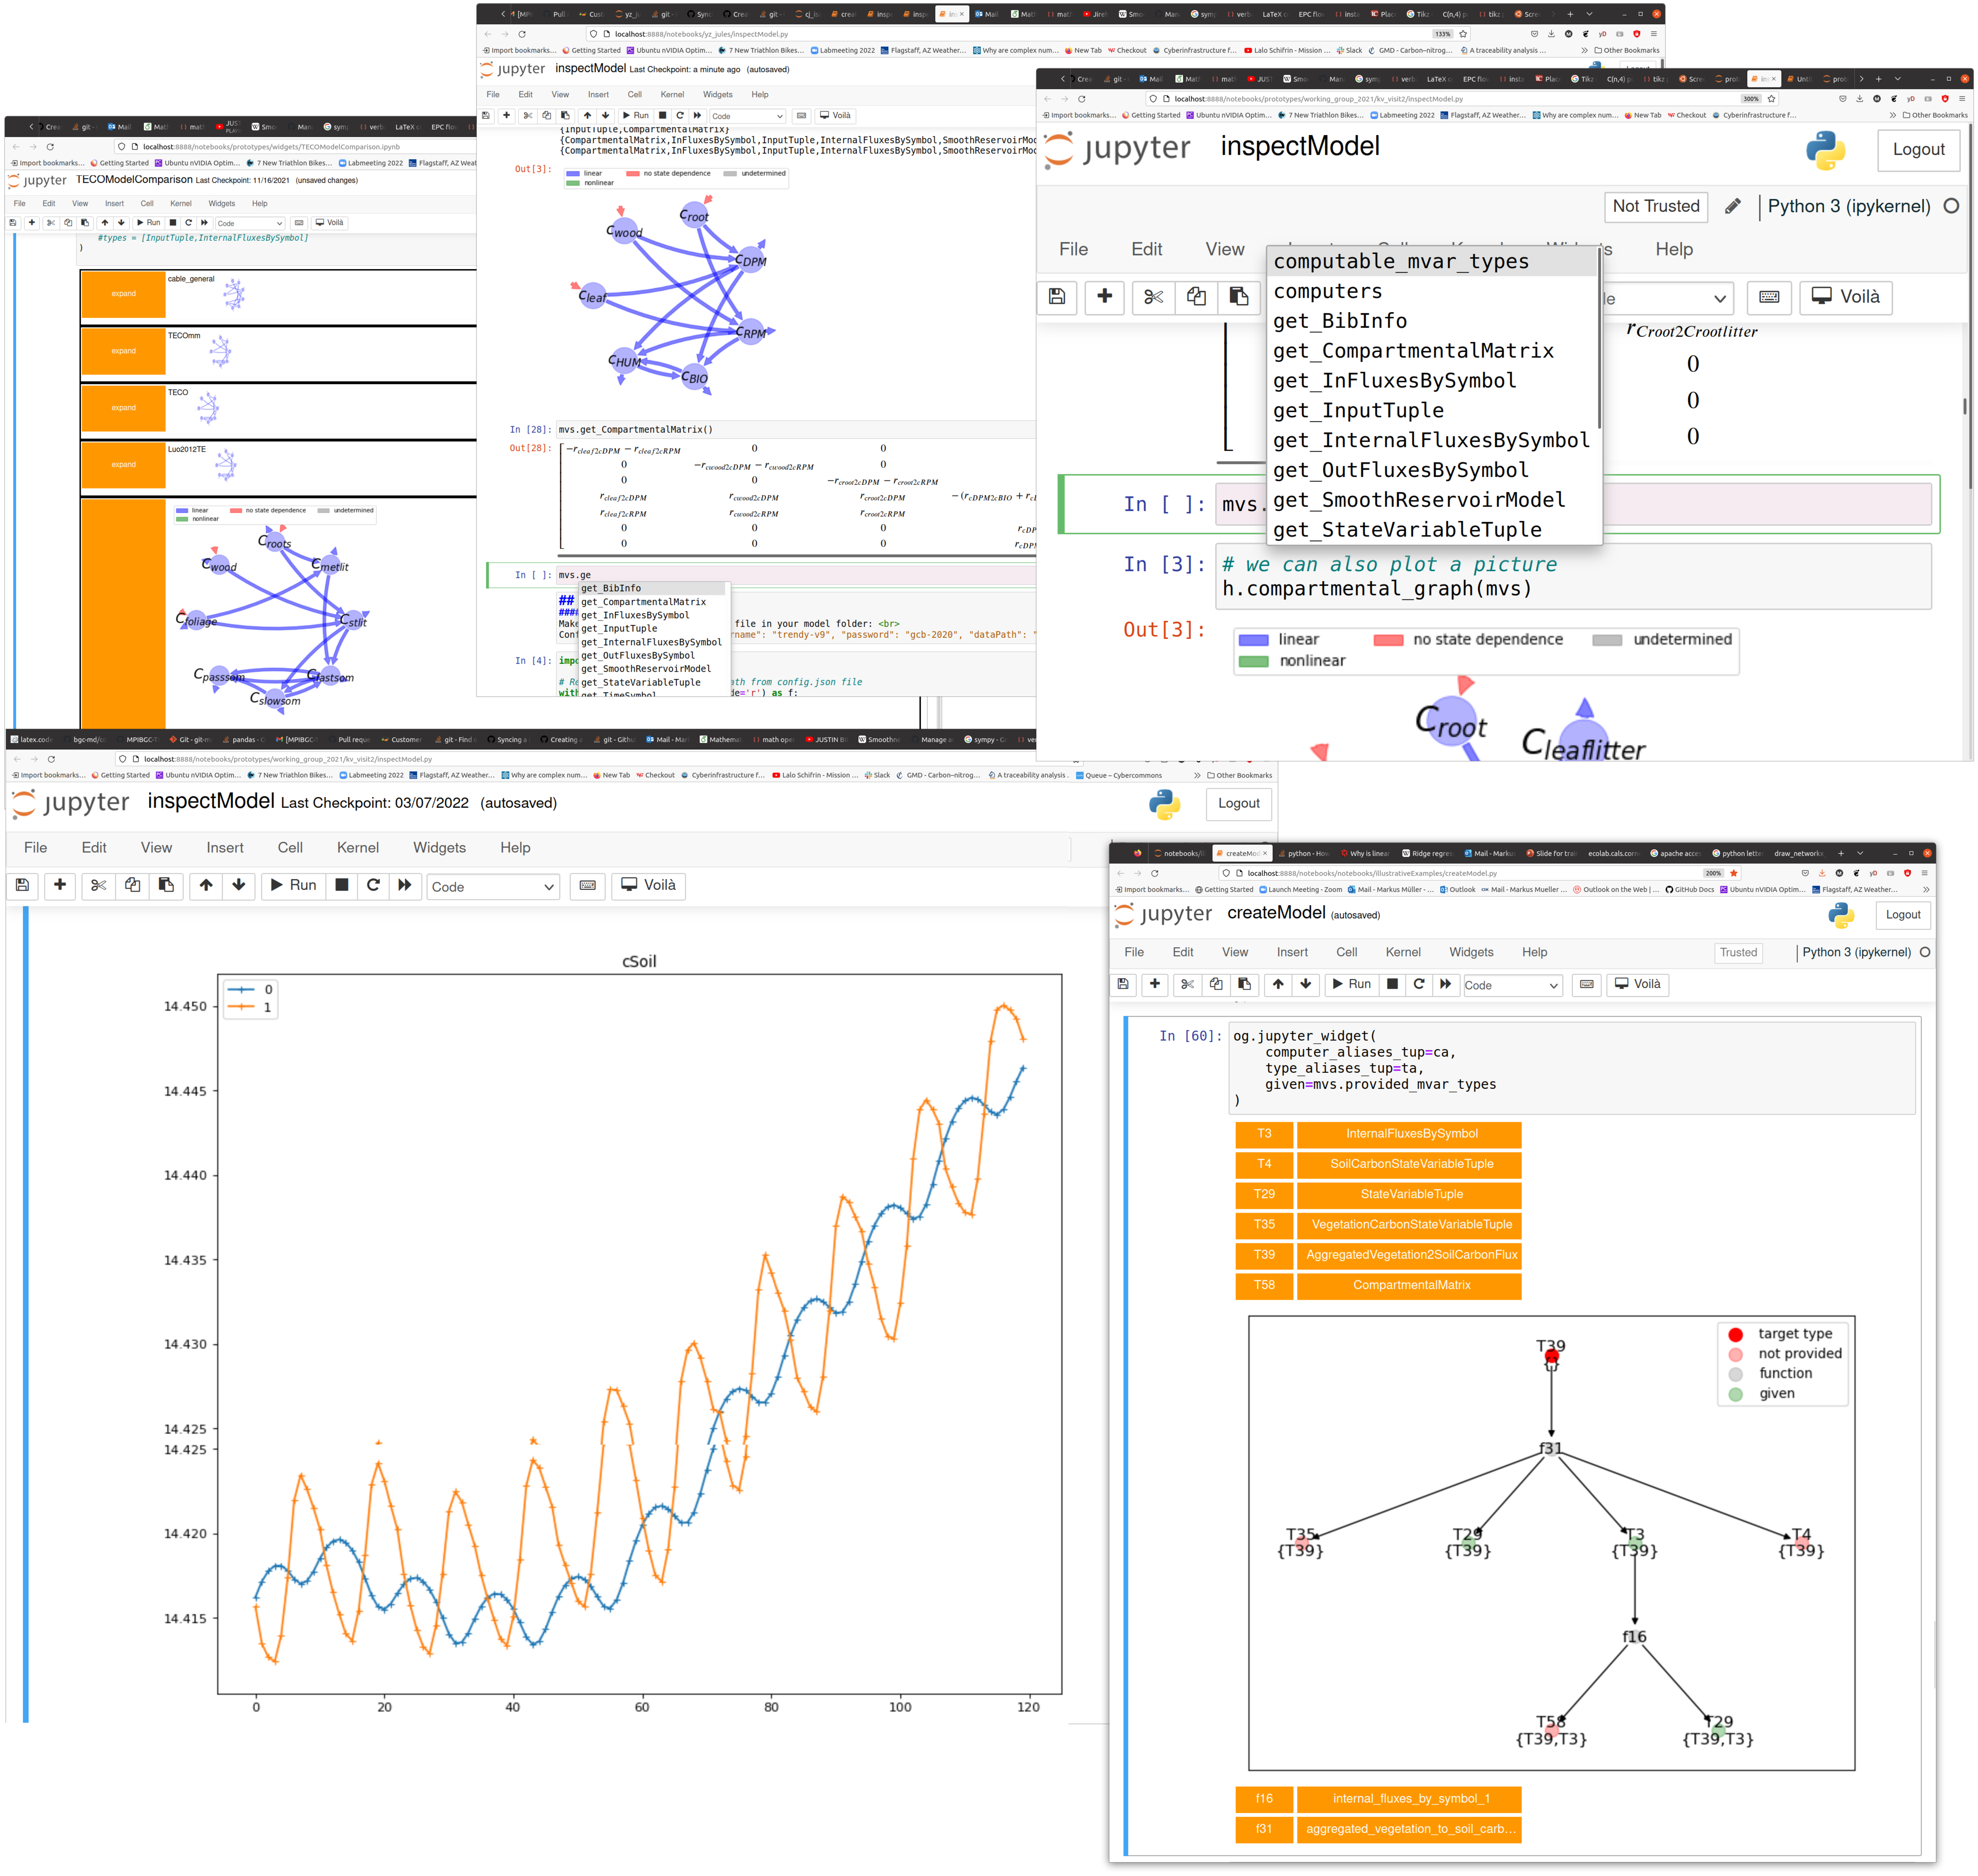
\includegraphics[width=\columnwidth]{TabScreenCombined.pdf}
	  \begin{itemize}
      \item Figure description, top row, left to right: 
	    \begin{itemize}
	      \item 
        Interactive jupiter widget with a table of models (orange buttons can be clicked to 
	      expand or collape a more detailed view of the particular model),
	      \item 
	      Model inspection with pool connection graph, which can be derived from the symbolic description
	      along other symbolic properties as flux equations and the compartmental matrix,
	      \item 
        Zoom into IPython/Jupyter UI, showing methods automatically added by the computability graph library. 
	    \end{itemize}
    \item Bottom row:  
	    \begin{itemize}
	      \item 
        Data assimilation with an automatically created numeric model (from symbolic description), 
	      \item 
        Computability graph for a desired diagnostic (aggregated Flux from the vegetation to soil part, showing 
        that the additionally needed information to compute the desired result)
	    \end{itemize}
	  \end{itemize}
}

%%%%%%%%%%%%%%%%%%%%%%%%%%%%%%%%%%%%%%%%%%%%%%%%%%%%%%%%%%%%%%%%%%%%%%%%%%%%%%%%%%%%%----
%\posterbox[adjusted title=Training Course]
%    {
%    name=course,
%    %column*=4,
%    column=1,
%    below=overview,
%    }{
%\begin{center}
%	  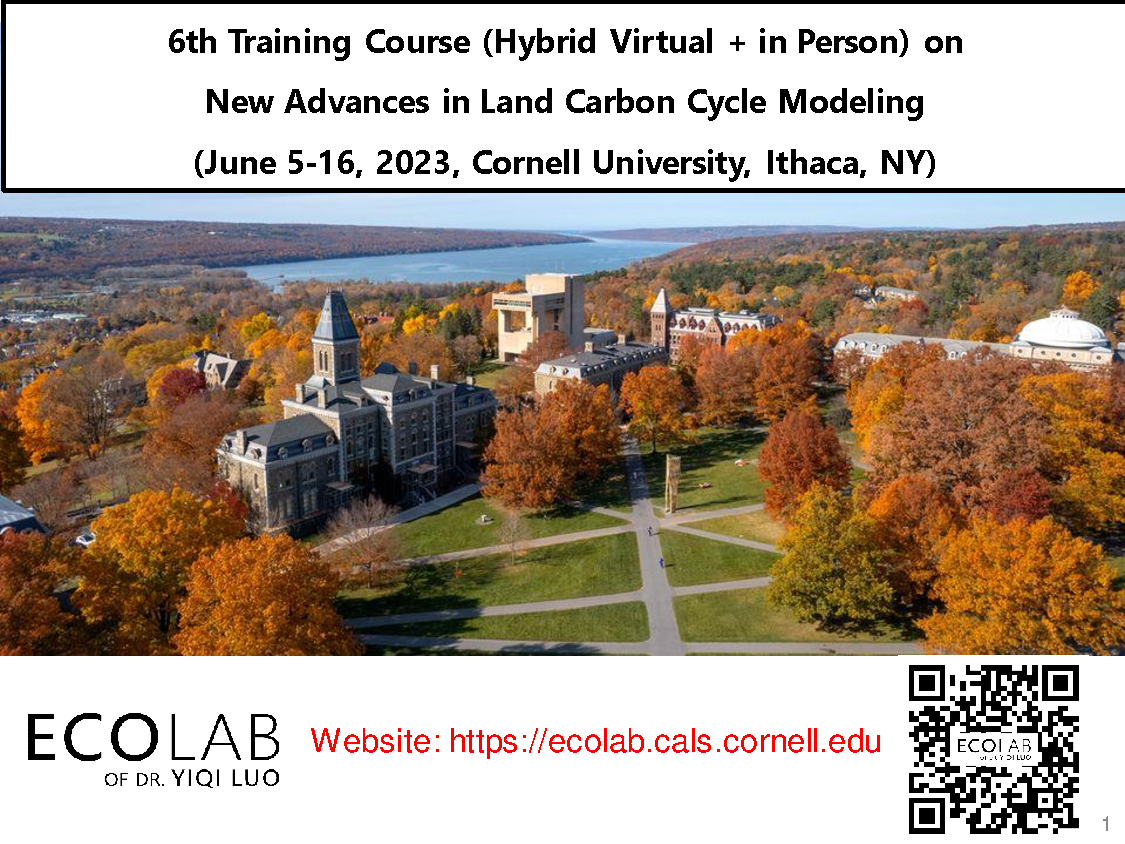
\includegraphics[width=.9\textwidth]{Slide_for_training_course.pdf}
%\end{center}
%}

%%%%%%%%%%%%%%%%%%%%%%%%%%%%%%%%%%%%%%%%%%%%%%%%%%%%%%%%%%%%%%%%%%%%%%%%%%%%%%%%%%%%%----
\posterbox[adjusted title=Model Inter Comparison]{
  name=ModelIntercomparison,
  column=2,
  span=2,
  below=title,
  %rowspan=2,
  %sequence=1 between overview and bottom then 2 between title and bottom
  }{
\begin{multicols}{2}
\begin{center}
  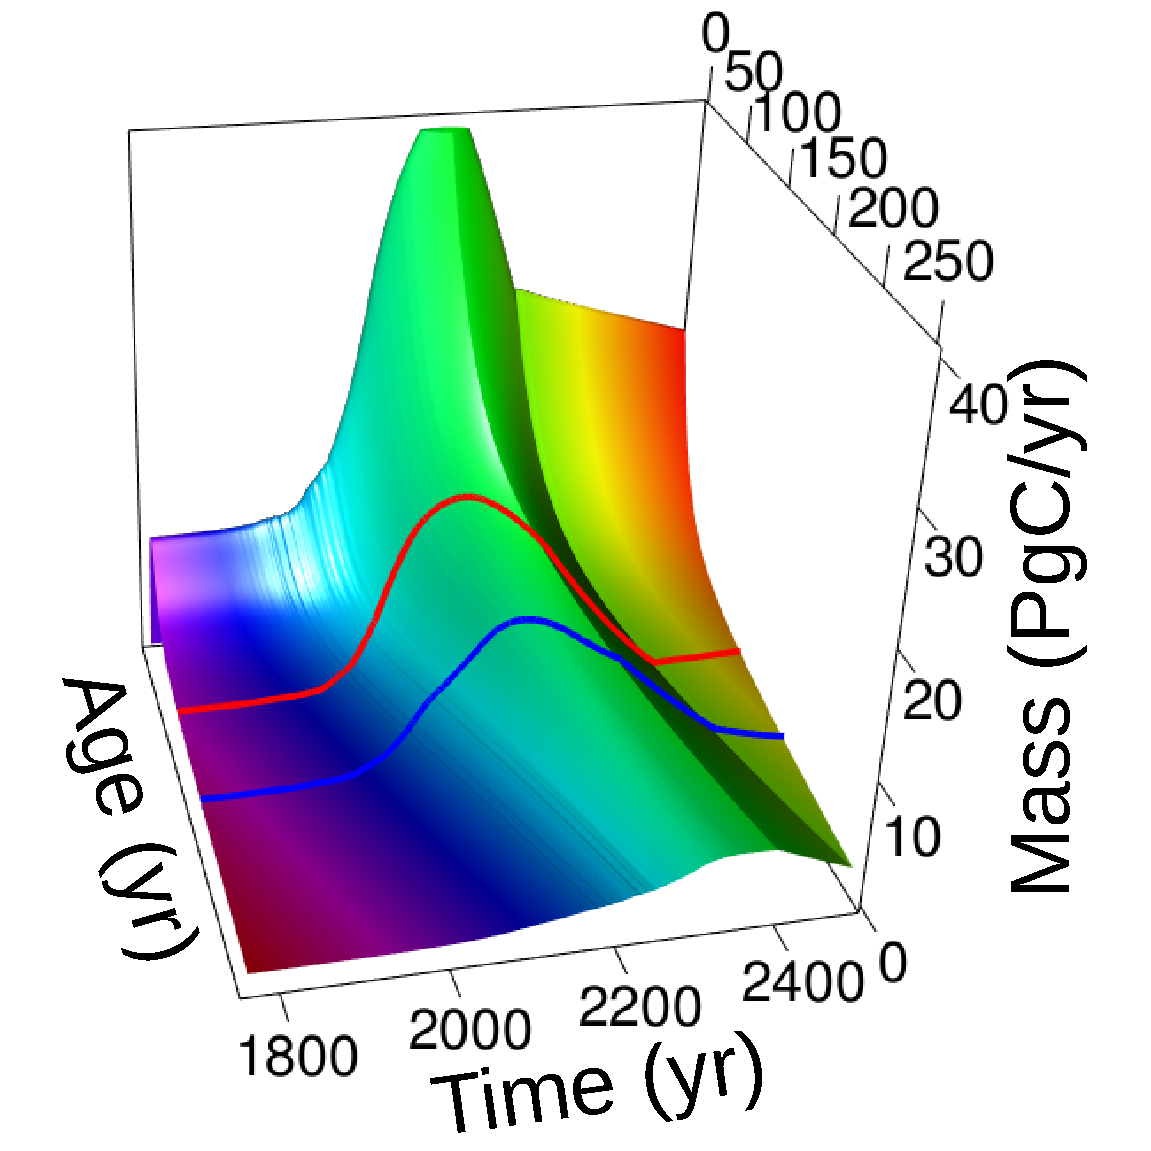
\includegraphics[width=\columnwidth]{atmosphere_nonlinear.pdf}
Figure above: System age distribution for a pool in a compartmental carbon cycle model
\end{center}
\begin{center}
	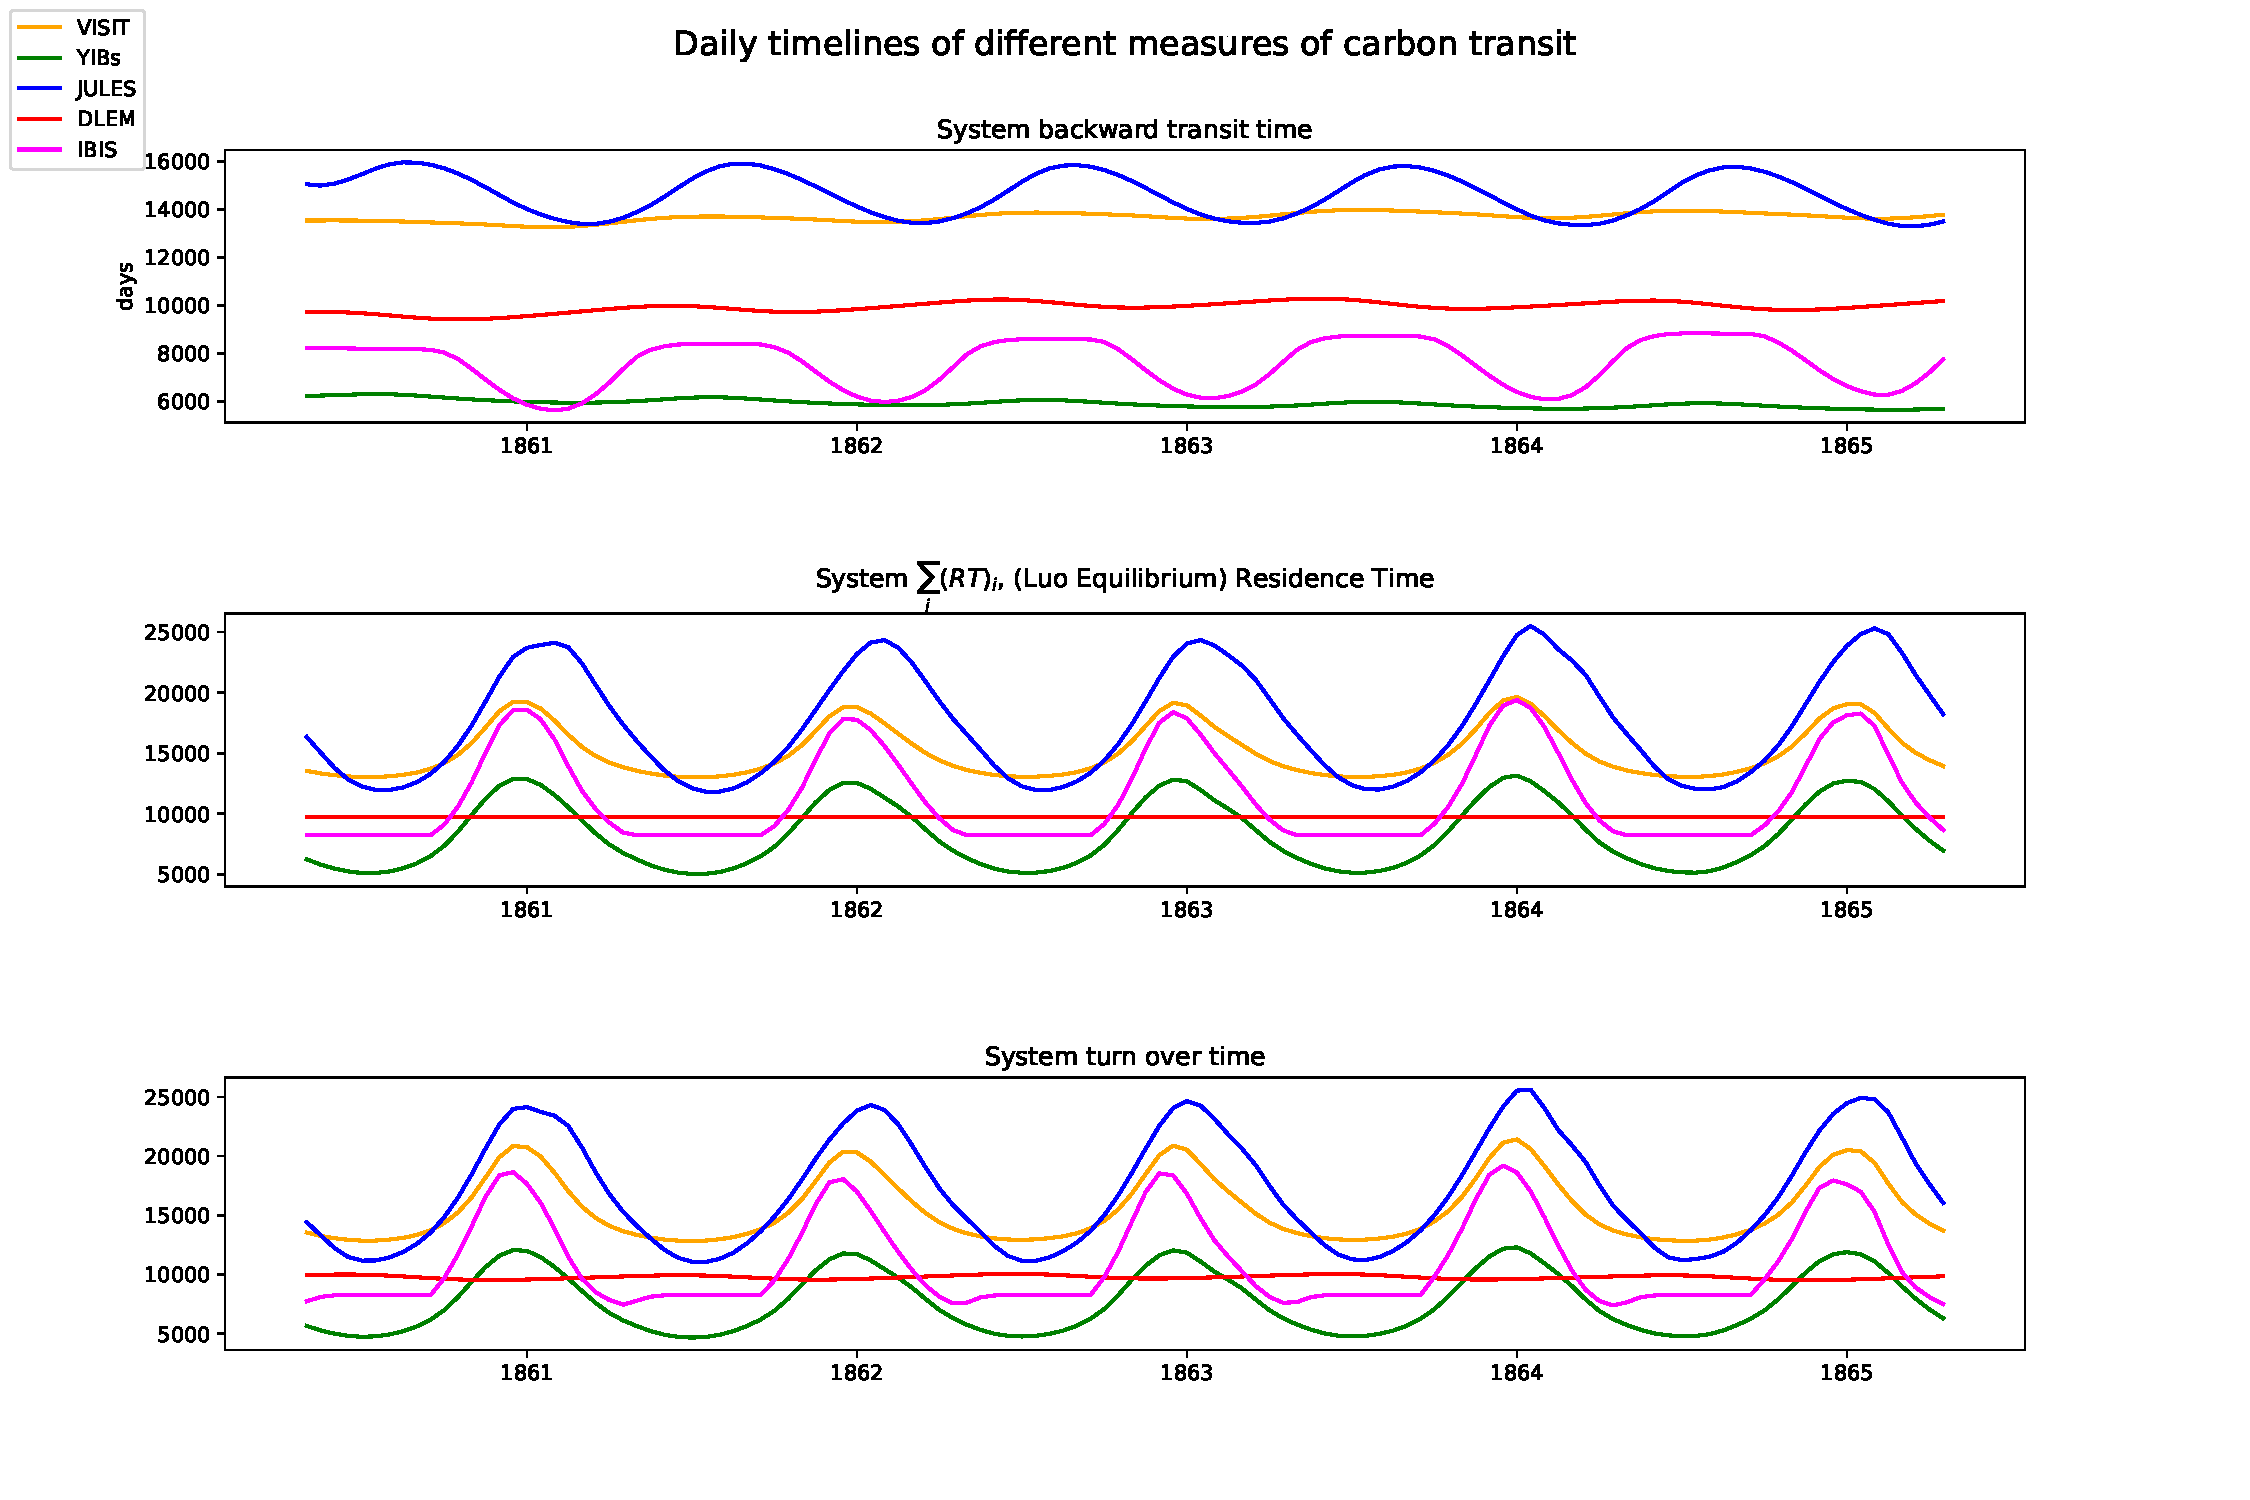
\includegraphics[width=\columnwidth]{test.pdf}
  Figure above: Comparing three different measures of transit time for five different models, using
  model reconstructions from trendy data.
\end{center}

\begin{minipage}[b]{\linewidth}
\begin{center}
	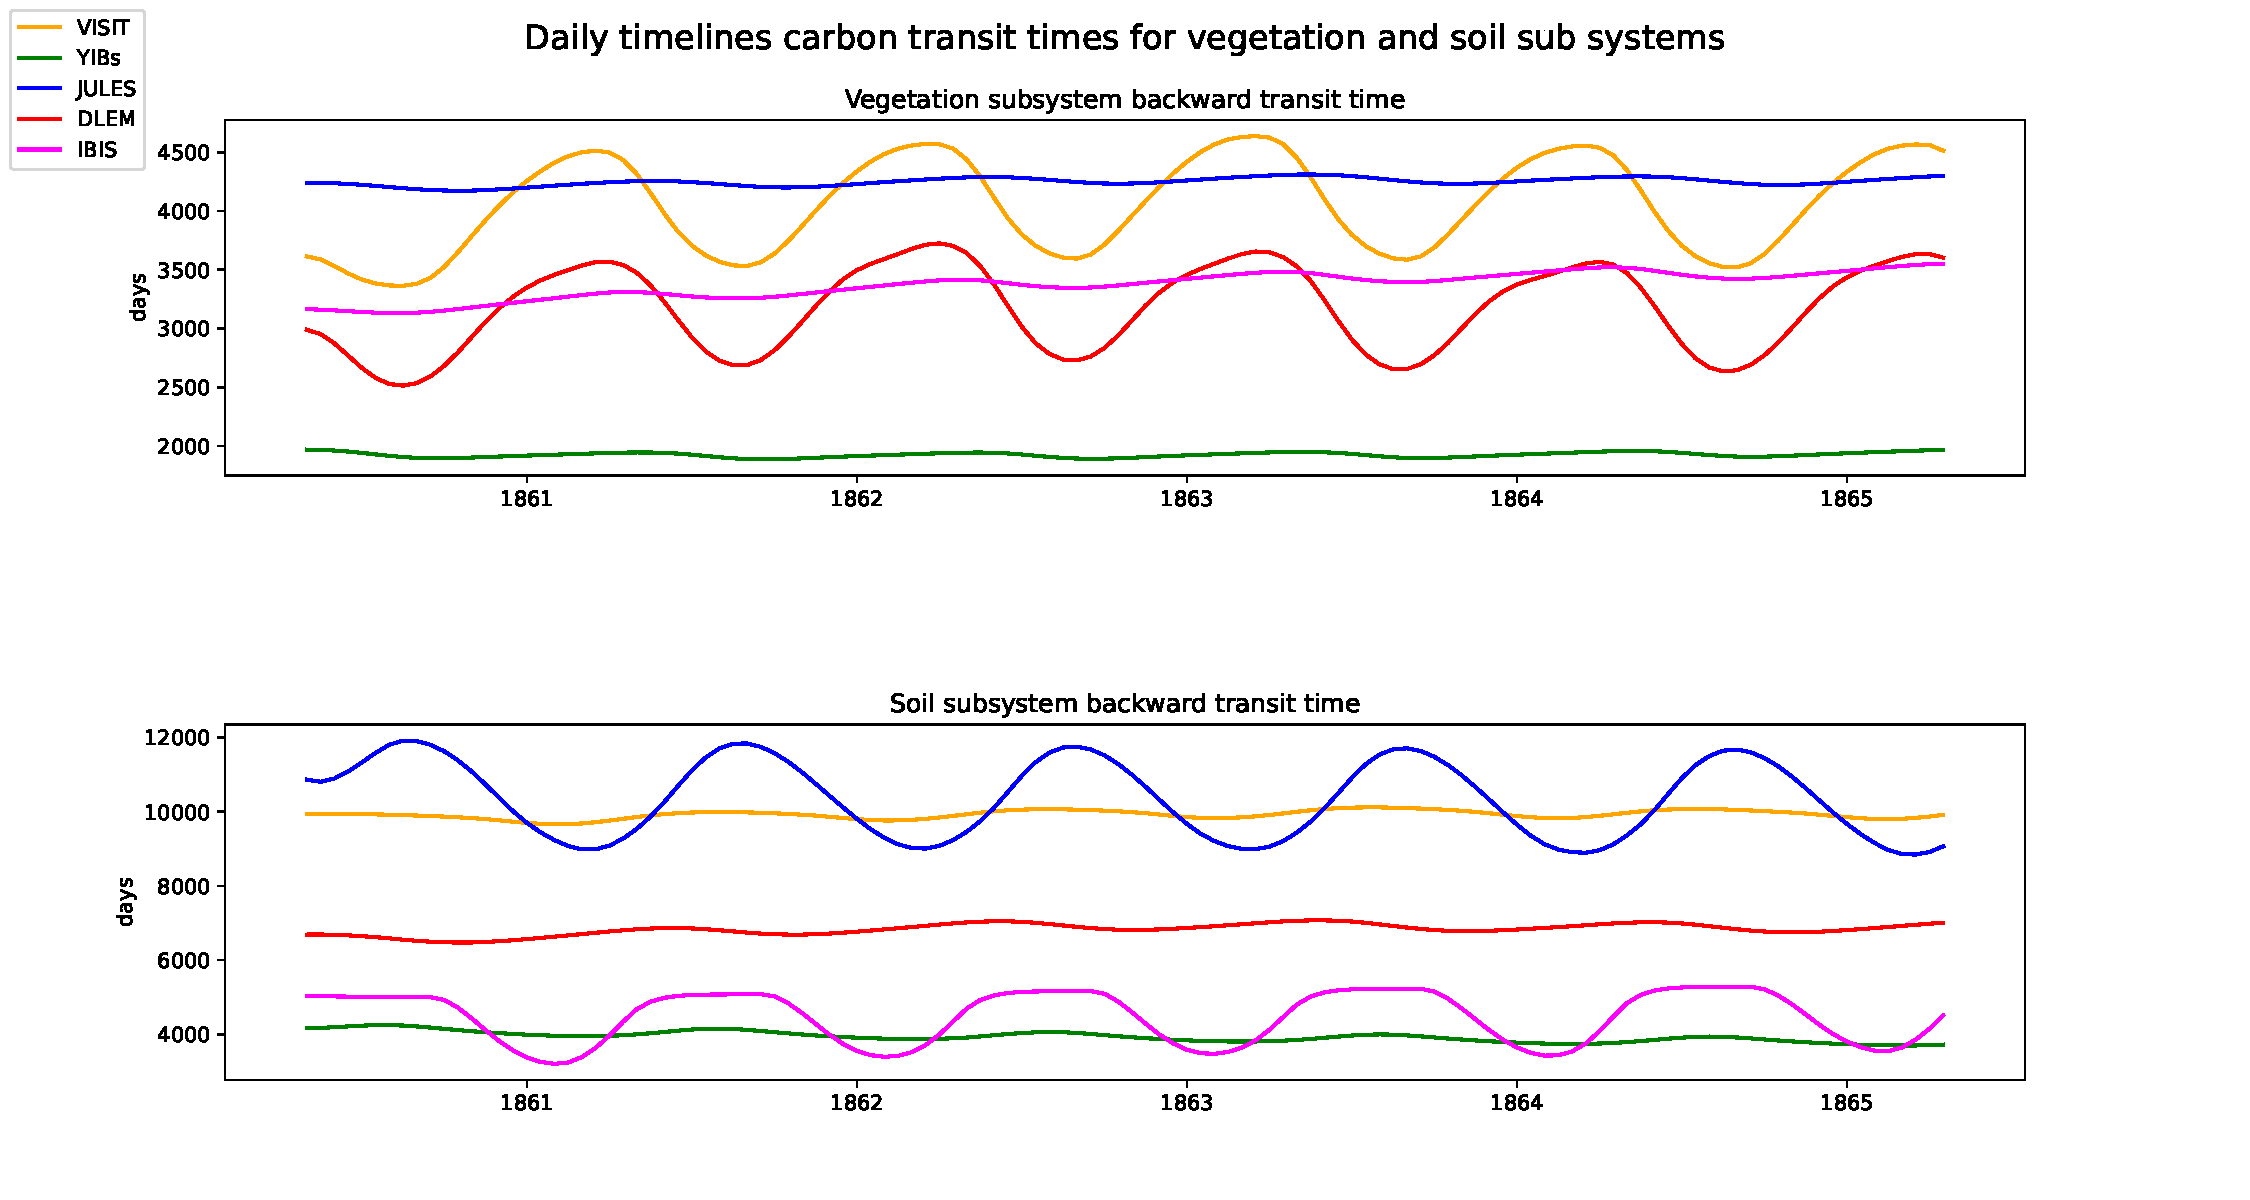
\includegraphics[width=\columnwidth]{test_veg_soil.pdf}
  Figure above: Comparing the (real = transient) backward transit time through 
  subsystems, accross different models. 
\end{center}
\end{minipage}

\begin{center}
	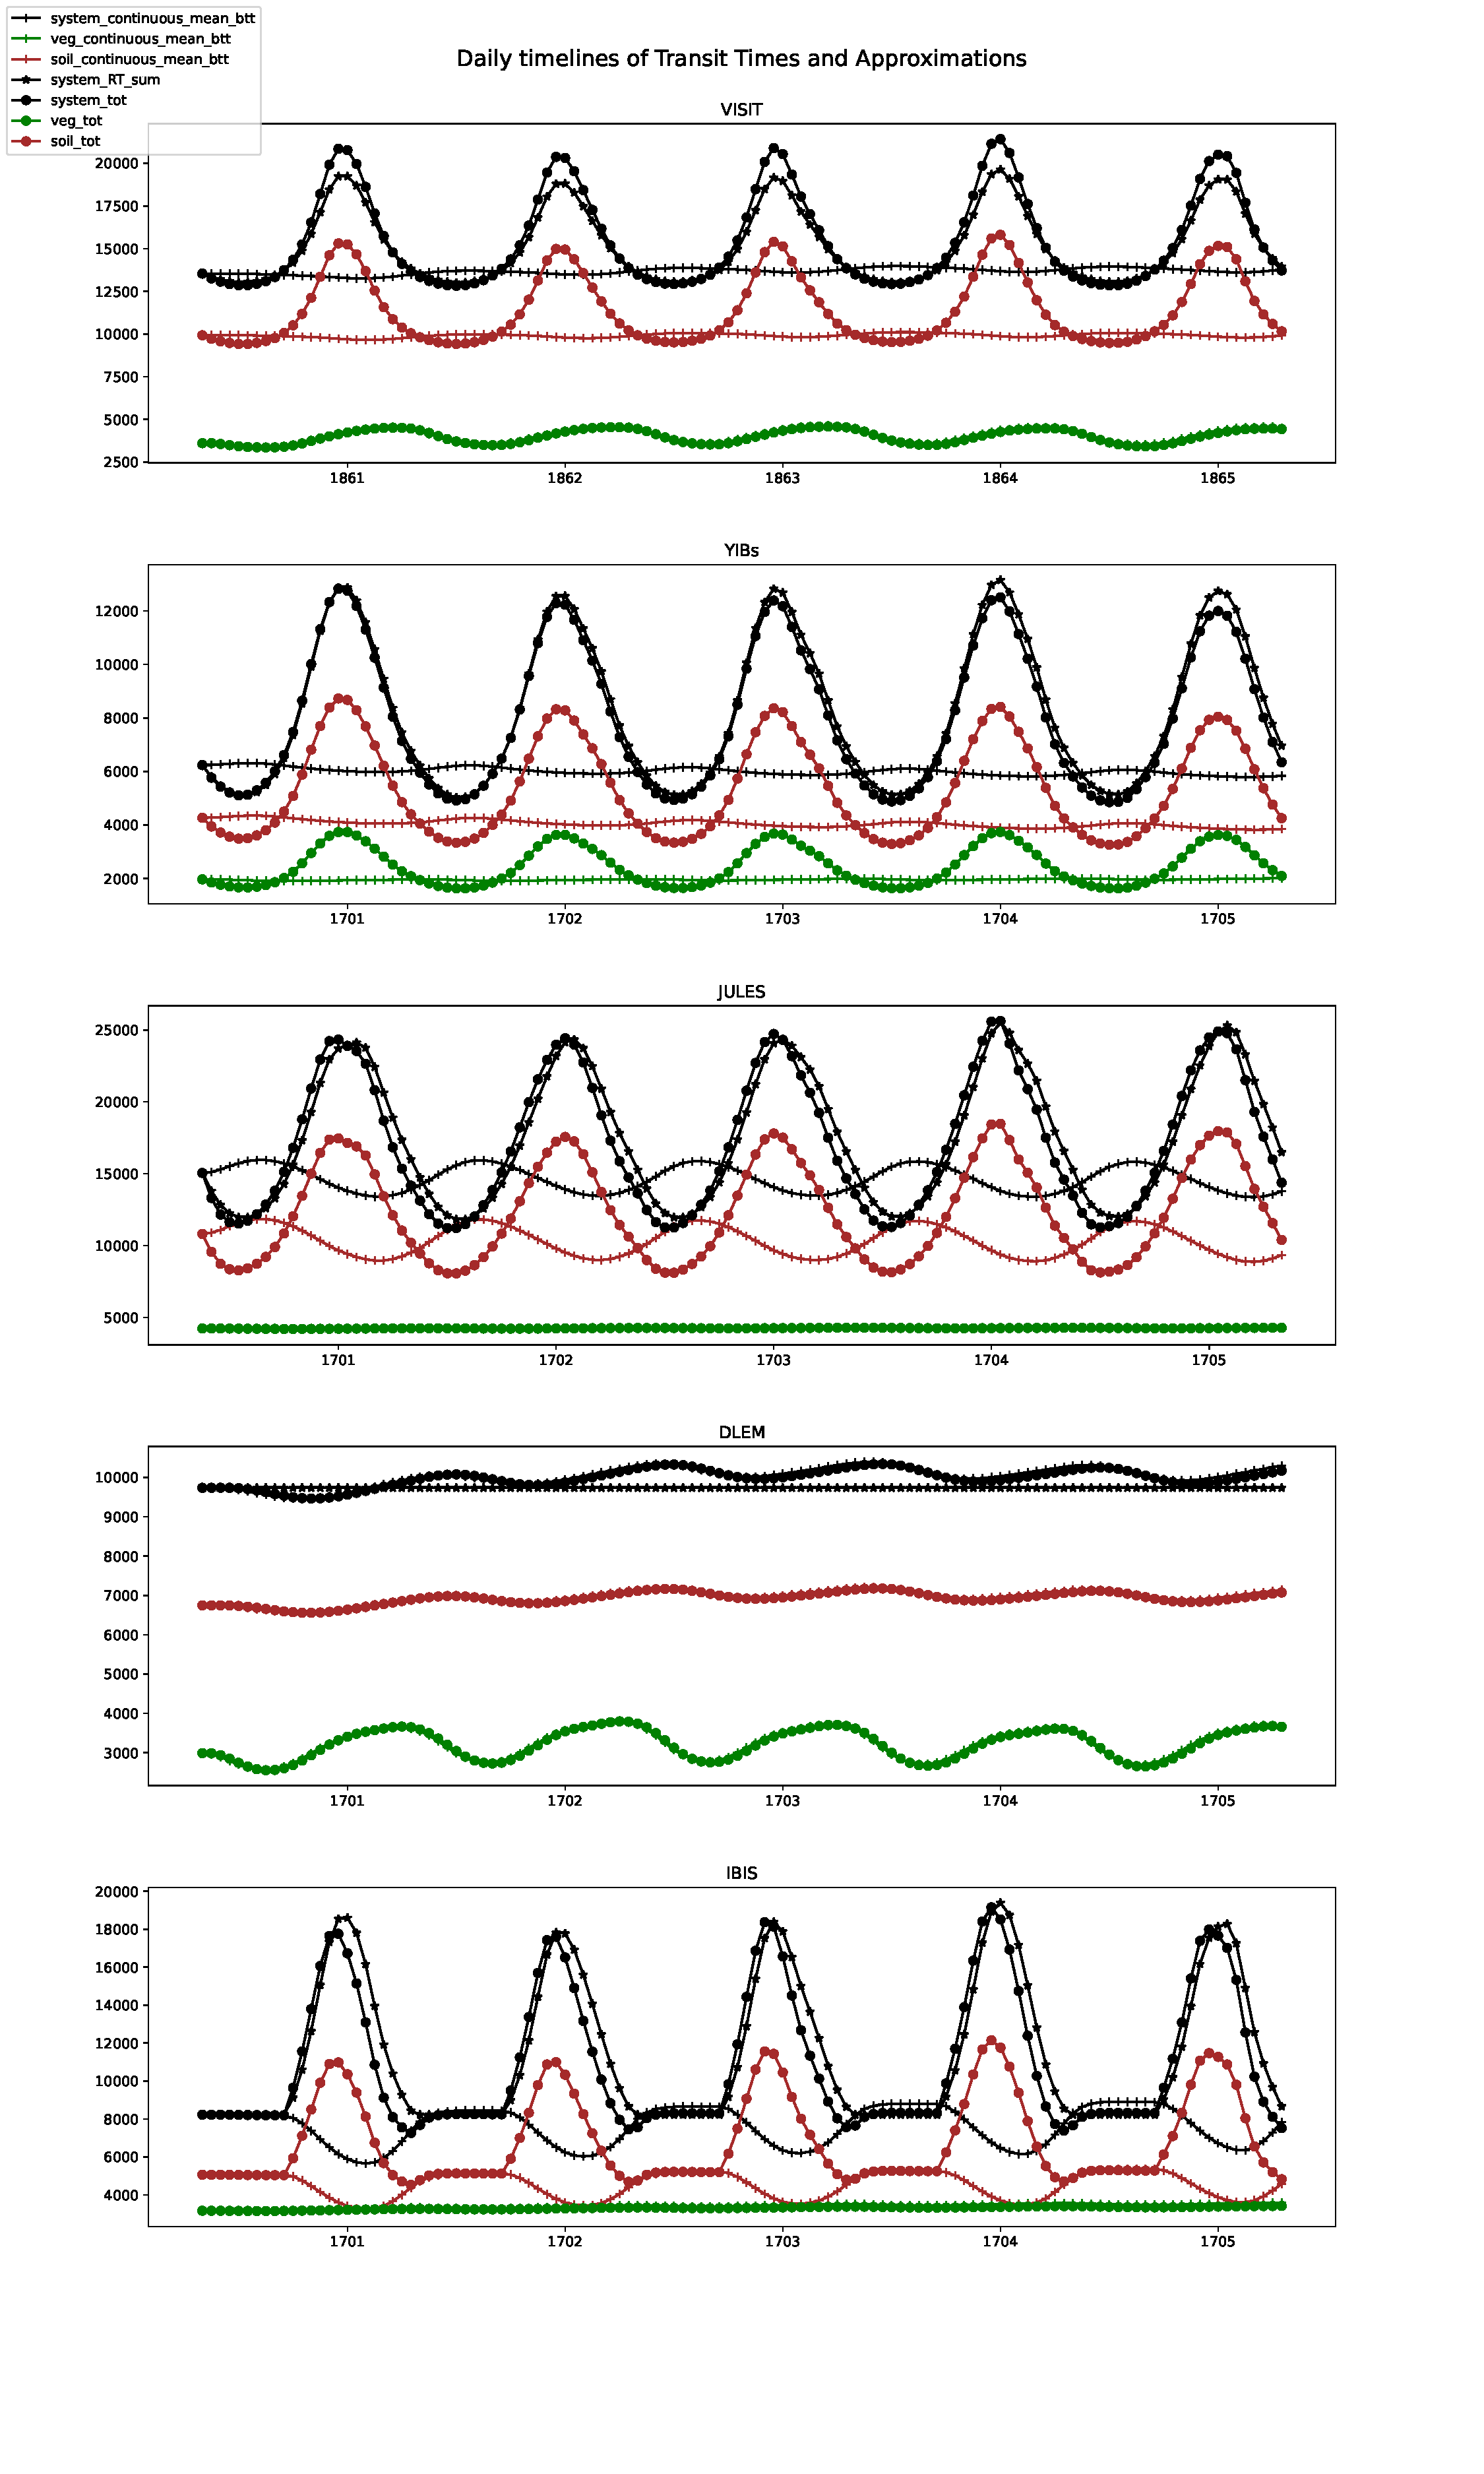
\includegraphics[width=\columnwidth]{test2_fine.pdf}
  Figure above: Another possible diagnostic plot: All tranist time measures together for every model.
  One model (DLEM) shows a very different behaviour.
\end{center}
\begin{center}
	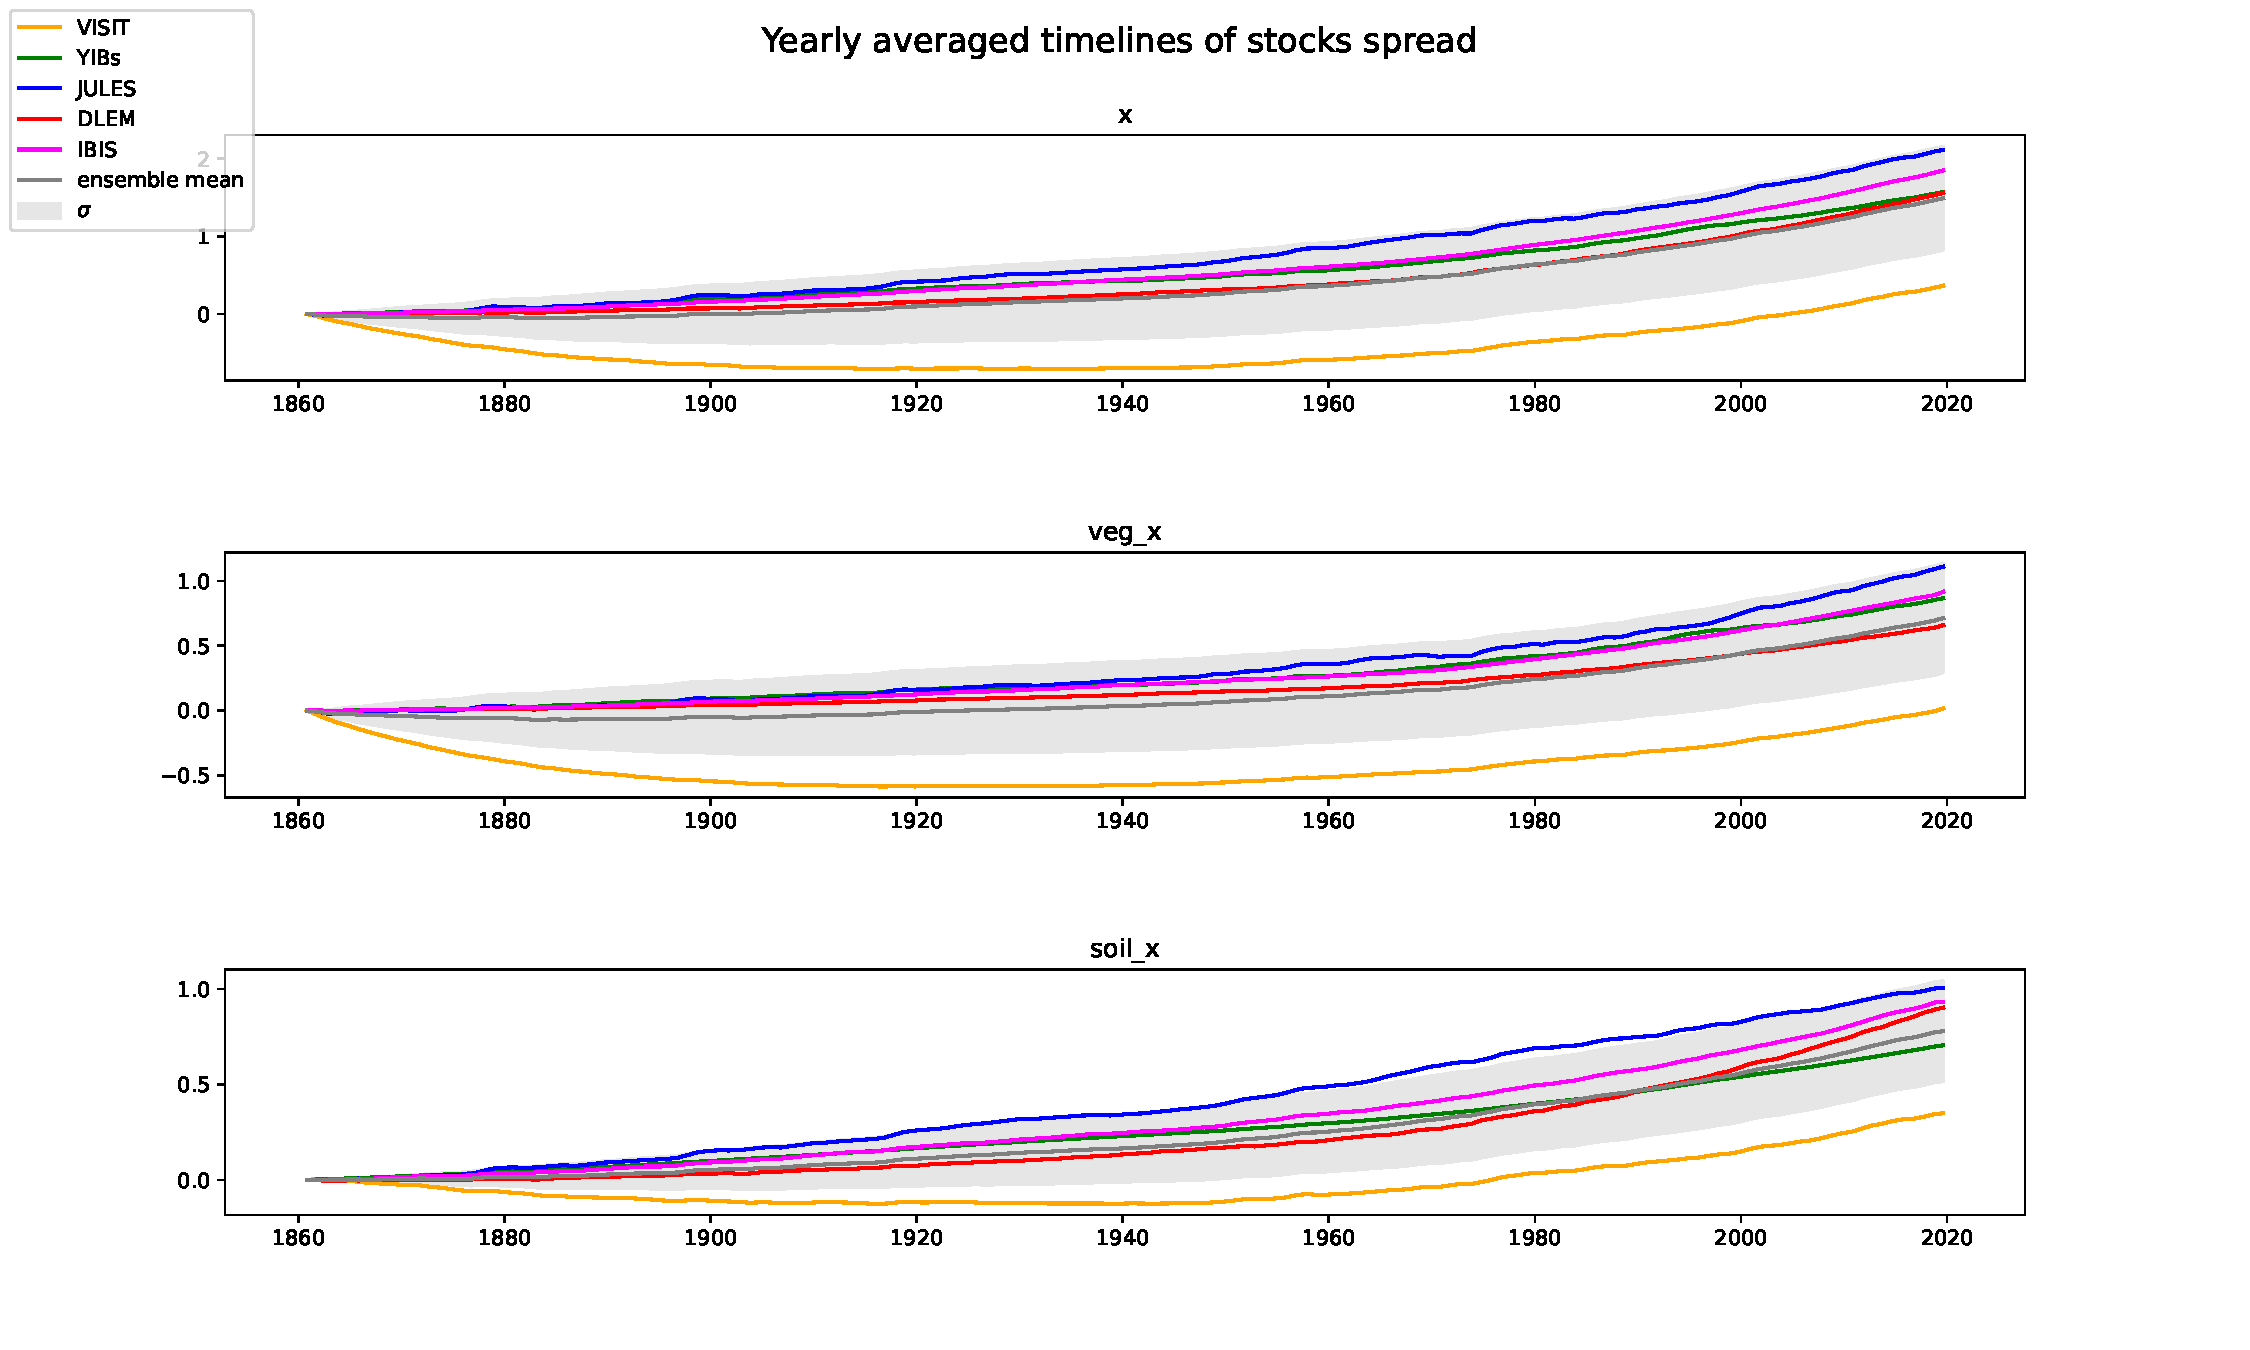
\includegraphics[width=\columnwidth]{test_stock_mean.pdf}
  Figure above: Total Carbon stock and subsystem stock development for different models.
  \texttt{bgc\_md} only needs to be told which pools belong to which subsystem.
\end{center}

\subsubsection*{Many diagnostics for many models}
\begin{itemize}
\item
  Many diagnostics (including those that are difficult to implement) available to all models 
\item
  Focus on model properties by exclusion of algorithmic differences
  (diagnostics for all models are computed by the same function )
\item
  Higher reliability (>100 unittests for many parts of the library, newly discovered errors have to be fixed
  only once)

   
\end{itemize}
  
  %%%%%%%%%%%%%%%%%%%%%%%%%%%%%%%%%%%%%%%%%%%%%%%%%%%%%%%%%%%%%
  \subsubsection*{References}
  \nocite{Luo2017Biogeosciences}
  \nocite{Rasmussen2016JMB}
  \nocite{Metzler2018PNAS}
	%\begin{thebibliography}{}
	%\bibitem[Metzler, Müller, Sierra, 2018]{Metzler2018PNAS}
	%Metzler, H., M{\"u}ller, M., and Sierra, C. (2018).
	%\newblock Transit-time and age distributions for nonlinear time-dependent
	%  compartmental systems.
	%\newblock {\em Proceedings of the National Academy of Sciences}, 115:201705296.
	%\end{thebibliography}
  \tiny{
  \bibliographystyle{abbrvnat}
  \bibliography{TEE-clean.bib}
  }
\end{multicols}


}

%%%%%%%%%%%%%%%%%%%%%%%%%%%%%%%%%%%%%%%%%%%%%%%%%%%%%%%%%%%%%%%%%%%%%%%%%%%%%%%%%%%----
\posterbox[adjusted title=Transparent Source Code]{
  name=code,
  %column*=4,
  column=4,
  %sequence=3 between title and bottom then 4 between top and record
  below=title,
  %column=2,
  %span=1.5,
  %above=bottom
  }{
  
%\section*{Structure} 
\subsubsection*{Integration with python tools }
  \begin{itemize}
  \item
   Build around and usable with other \texttt{python} tools,( \texttt{DASK, Jupyter, NumPy, SciPy, SymPy,NetworkX\dots}). 
  \item 
  Only open source dependencies inside the python universe.
  \item 
  Thin frontend for other packages developed at the Max-Planck-Institute in Jena.
    \begin{itemize}
    \item
        Computability graph computation outsourced into \texttt{ComputabilityGraphs} 
    \item
	    Advanced diagnostic variables (age and transittime distributions) 
      provided by \texttt{LAPM} and \texttt{CompartmentalSystems} 
    \end{itemize}
  \end{itemize}
  \begin{center}
  \begin{tikzpicture}[sibling distance=27em,
    every node/.style = {shape=rectangle, rounded corners,
      draw, align=center,
      top color=white, bottom color=red!20}]
      \node {
      \begin{tikzpicture}[anchor=center]
        \node {
        \texttt{bgc\_md2}
        }
        child { node {\texttt{ComputabilityGraphs}} }
  	    child { node[sibling distance=3em]{\texttt{CompartmentalSystems}}
  	    child { 
          node (LAPM){\texttt{LAPM}}
        }
  	    %child [level distance=3em]{ node (SymPy){\texttt{SymPy}} }
  	    %child [level distance=3em]{ node (NymPy){\texttt{numpy}} }
      };
  	%\draw[->] (LAPM) -- (SymPy); 
    \end{tikzpicture}
    };
  \end{tikzpicture}
  \end{center}

  %%%%%%%%%%%%%%%%%%%%%%%%%%%%%%%%%%%%%%%%%%%%%%%%%%%%%%%%%%%%%%
  \subsubsection*{Internal Structure}
  \begin{itemize}
    \item
      A collection of models, organized as subpackages
  \begin{center}
  \begin{tikzpicture}[%sibling distance=38em,
    every node/.style = {shape=rectangle, rounded corners,
      draw, align=center,
      top color=white, bottom color=red!20}]]
    \tikzstyle{level 1}=[sibling distance=25.5em]
    \tikzstyle{level 2}=[sibling distance=5em]
    \tikzstyle{level 3}=[sibling distance=3em]
    \tikzstyle{level 4}=[sibling distance=1.75em]
      \node {% <- this 'right of' is inherited; how to avoid?
      \begin{tikzpicture}[anchor=center]
        \node {\texttt{bgc\_md2}
        %\draw (0,0) -- (0,1);
        %\node[fill] at (0,.5) {};
        } 
        child{ node {models}
  	 child{ node{rothC}
  	    child{node {Fluxes}}
  	    child{node {Pools}}
  	    child{node {\dots}}
  	}
        	child{ node {Wang}
  	%    child{node {Fluxes}}
  	%    child{node {Pools}}
  	%    child{node {\dots}}
  	}
        	child{ node {\dots}}
        }
        child{ node {computers}
  	 child{node {Matrix(Fluxes)}}
  	 %child{node {Fluxes(Matrix,Pools)}}
  	 child{node {\dots}}
        };
      \end{tikzpicture}
      };
  \end{tikzpicture}
  \end{center}
    \item 
      Formulated as (arbitrarily small) sets of varibles of specific type, using 
    \item 
      A collection of special domain specific datatypes (like influxes or compartmental matrix), connected by
    \item
      A set of type annotated functions (computers), forming a network of computability.
    \item
      A central class \texttt{CMTVS} (ConnectedMultytypeVariableSet) facilitating the recursive derevation
      of computable properties.
    \item
      Some helpers to interface with other packages e.g. enhancing the jupyter UI
  \end{itemize}

  %%%%%%%%%%%%%%%%%%%%%%%%%%%%%%%%%%%%%%%%%%%%%%%%%%%%%%%%%%%%%
  %\subsubsection*{Database Records are \texttt{python} modules too}
  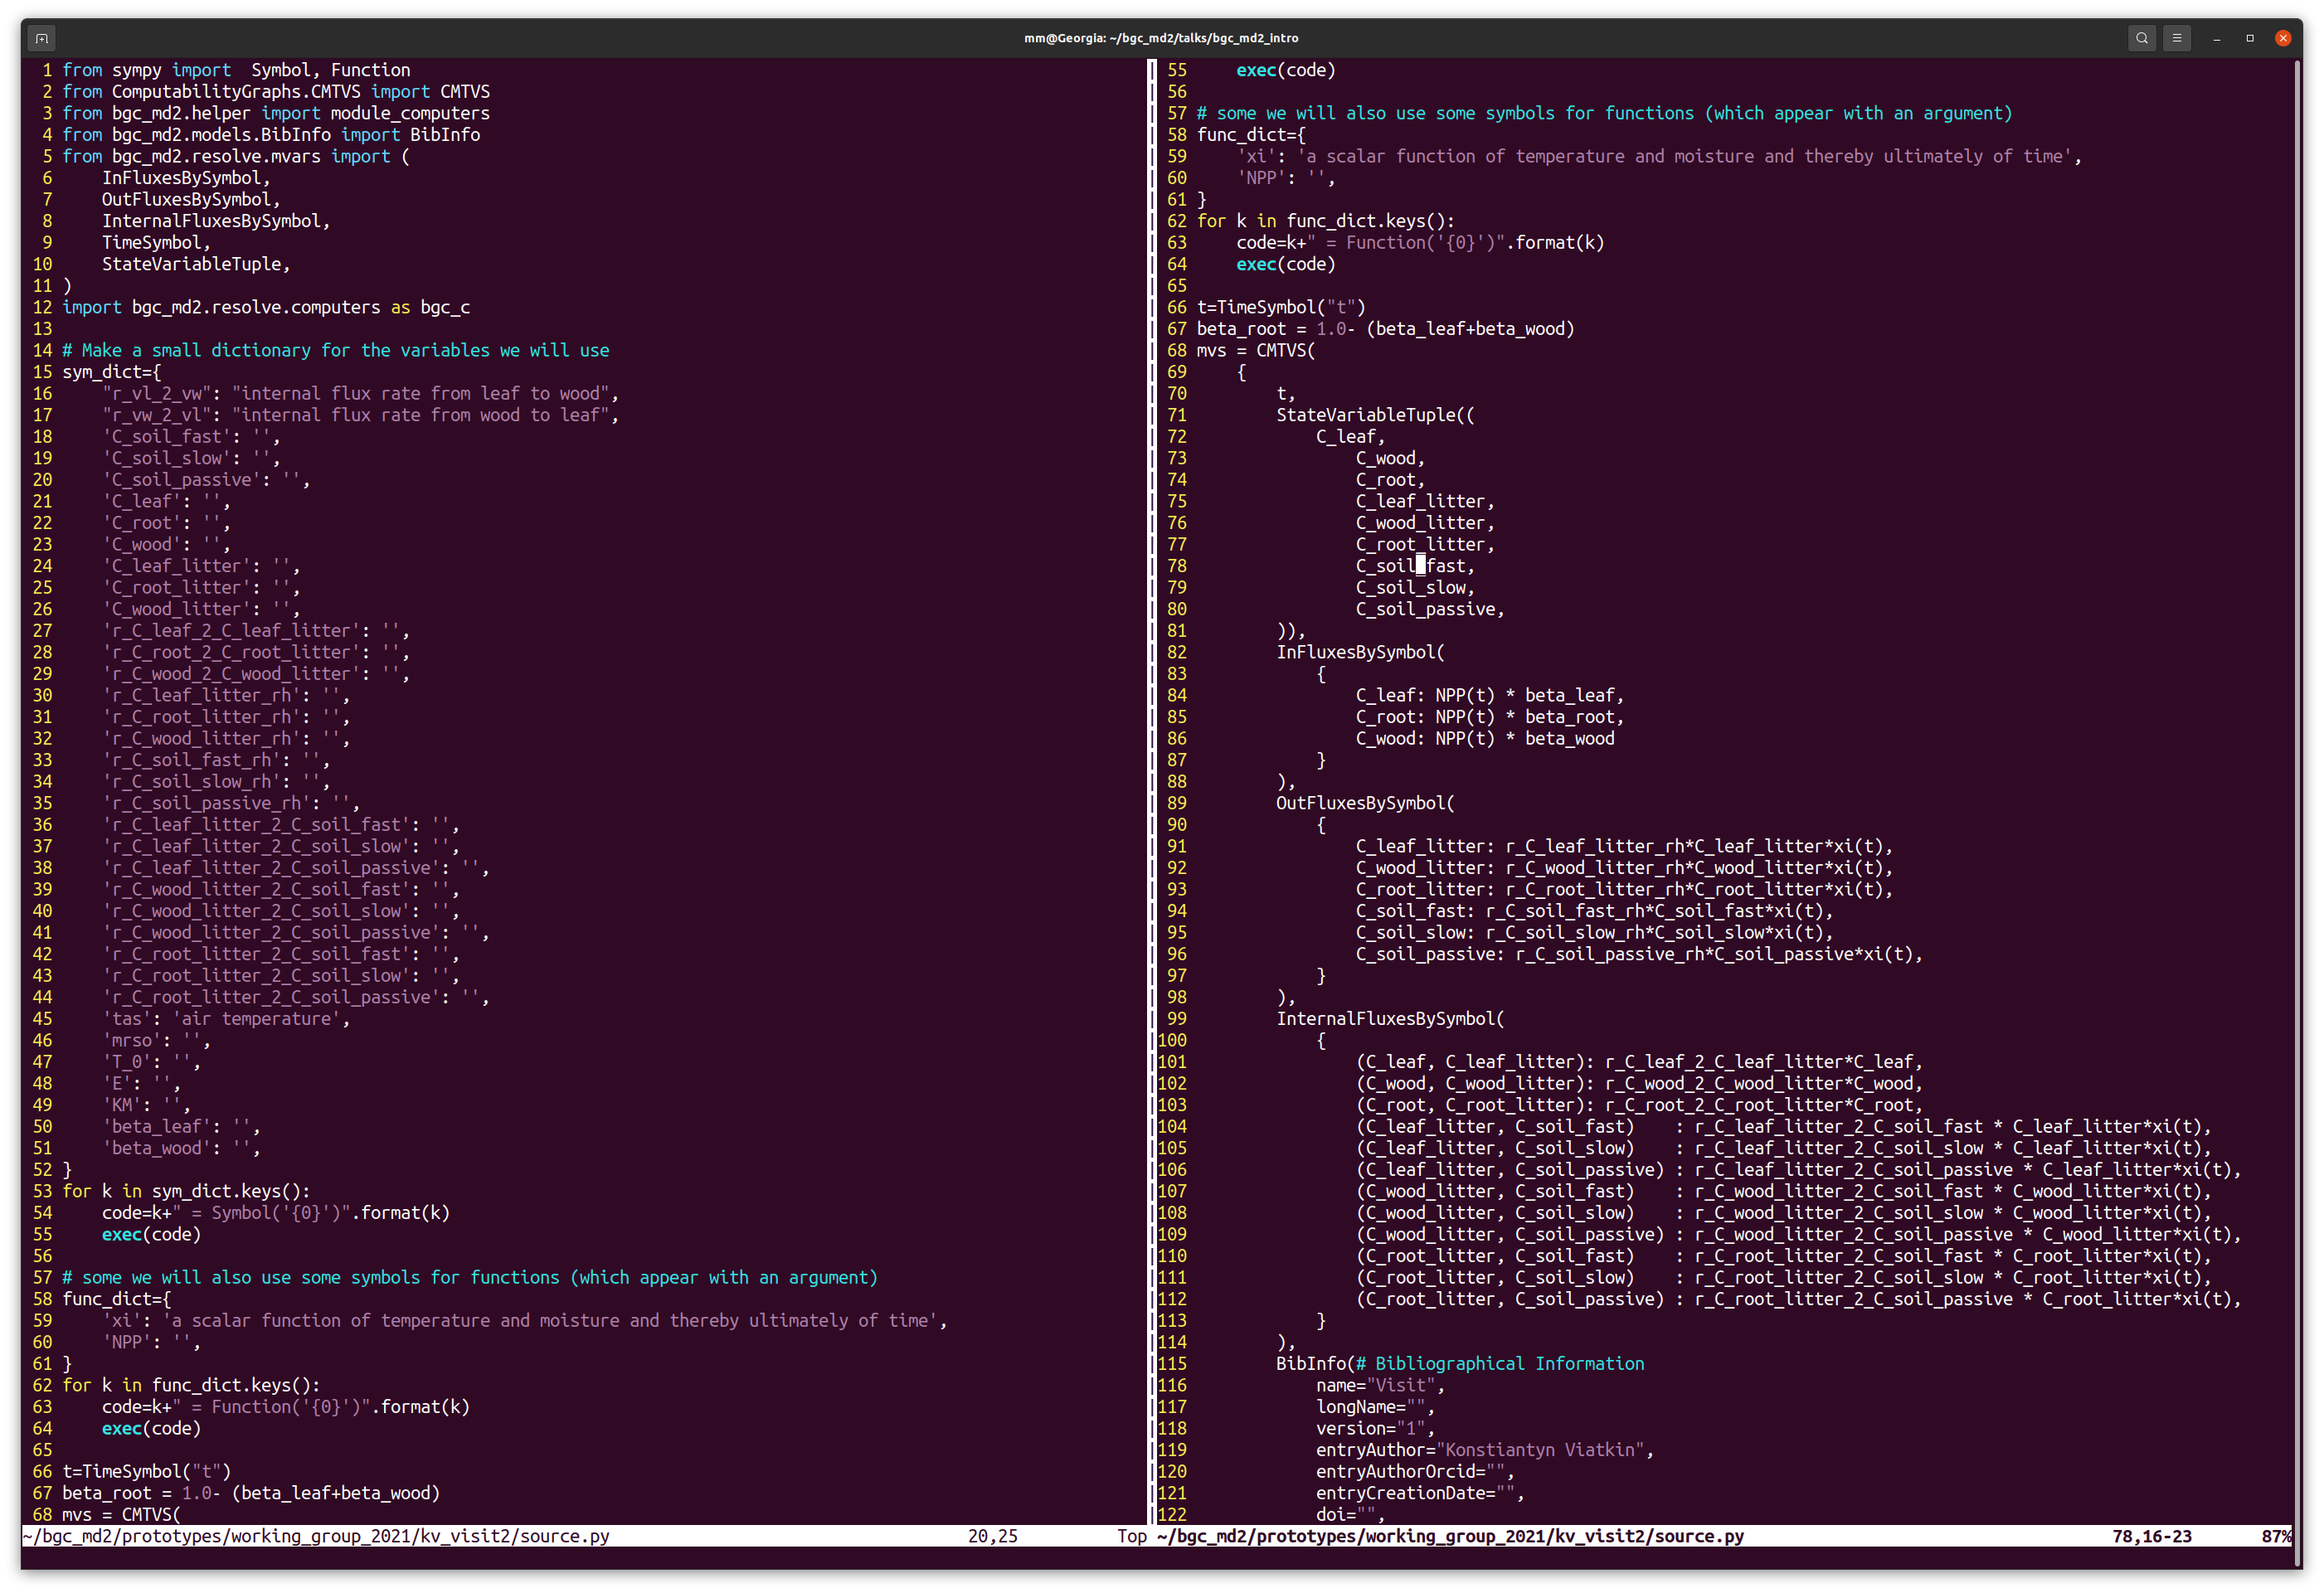
\includegraphics[width=\columnwidth]{source.py.png}
    Screenshot of the source code of the visit model using sympy and some datatypes provided by \texttt{bgc\_md2}
    to create a \texttt{CMTVS}  instance representing the model for comparisons.
     

  %%%%%%%%%%%%%%%%%%%%%%%%%%%%%%%%%%%%%%%%%%%%%%%%%%%%%%%%%%%%%
  \subsubsection*{To Do / Development/ Levels of contribution}
  \begin{itemize}
    \item Easy:
      Applcation of the existing functionality to more scientific questions and data,
      formulation of new models (including {\bf yours}), 
      improvement of the documentation (example notebooks, tests, and python docstrings)
    \item Medium:
      Implementation of new diagnostic variables and algorithms to compute them 
    \item Final:
      Integration of new building blocks and fucntions into the computability framework
      to make them much more easily accessible
  \end{itemize}
}
%%%%%%%%%%%%%%%%%%%%%%%%%%%%%%%%%%%%%%%%%%%%%%%%%%%%%%%%%%%%%%%%%%%%%%%%%%%%%%%%%%%%%----
%\posterbox[adjusted title=References]{
%  name=references,
%  %column*=4,
%  column=4,
%  below=code
%  %column=2,
%  %span=1.5,
%  %above=bottom
%  }{
%  \nocite{Luo2017Biogeosciences}
%  \nocite{Rasmussen2016JMB}
%  \nocite{Metzler2018PNAS}
%	%\begin{thebibliography}{}
%	%\bibitem[Metzler, Müller, Sierra, 2018]{Metzler2018PNAS}
%	%Metzler, H., M{\"u}ller, M., and Sierra, C. (2018).
%	%\newblock Transit-time and age distributions for nonlinear time-dependent
%	%  compartmental systems.
%	%\newblock {\em Proceedings of the National Academy of Sciences}, 115:201705296.
%	%\end{thebibliography}
%  \tiny{
%  \bibliographystyle{abbrvnat}
%  \bibliography{TEE-clean.bib}
%  }
%}
%%%%%%%%%%%%%%%%%%%%%%%%%%%%%%%%%%%%%%%%%%%%%%%%%%%%%%%%%%%%%%%%%%%%%%%%%%%%%%%%%%%%----
\posterbox[adjusted title=Connect]
    {
    name=contact,
    %column*=4,
    column=4,
    %below=ModelIntercomparison
    %below=references,
    below=code,
    }{
	  \includegraphics[height=3.2em]{qr_github.pdf}
    
    \href{https://github.com/MPIBGC-TEE/bgc\_md2\#readme}{Readme on github}
    \\
	  \includegraphics[height=3.2em]{qr_tutorial.pdf}
    \href{https://github.com/MPIBGC-TEE/bgc_md2/blob/test/notebooks/illustrativeExamples/createModel.ipynb}{A preliminary mini tutorial preview on github (in progress)}
    \\
	  \includegraphics[height=3.2em]{qr_mm.pdf}
    \href{mailto:markus.mueller.1.g@googlemail.com}{Main developer email address}
}
\end{tcbposter}
\end{document}

